\newcounter{Odvozeni}

Momentem hybnosti na první pohled nepůsobí jako téma, které by bylo pro chemika obzvláště palčivé. Ve skutečnosti je ale z~kvantové teorie pro chemika málo co důležitějšího. V~této kapitole se budeme zabývat výhradně orbitálním moment hybnosti~$\mathbf{L}$, spin  odsuneme do kapitoly \ref{kap:elektronovyspin}.  

Povídání o~momentu hybnosti začneme jeho definicí z~klasické mechaniky. Vybaveni aparátem základních kvantově mechanických operátorů -- polohy a hybnosti, odvodíme operátory pro moment hybnosti a komutační relace mezi nimi. Ukážeme, že když operátory komutují, znamená to, že mají společné vlastní funkce. Toho dále využijeme při řešení vlastního problému operátorů momentu hybnosti.

Pro popis rotačního pohybu nejsou příliš vhodné kartézské souřadnice. Zavedeme si proto vhodnější souřadné systémy a ukážeme, jaké výhody při řešení problémů s~momentem hybnosti poskytují. 

\subsection{Operátor momentu hybnosti}
\label{kap:OperatorMomentuHybnosti}

Z~klasické fyziky víme, že pohybující se částice o~hmotnosti $m$ rychlostí $v$ nese hybnost
\begin{equation}
p = mv \mbox{.}
\label{rov:Hybnost1}
\end{equation}
Rotace částice je spojena s~momentem hybnosti
\begin{equation}
\mathbf{L} = \mathbf{r} \times \mathbf{p} \mbox{,}
\label{rov:Hybnost2}
\end{equation}
kde $\mathbf{r}$ je pozice částice vůči zvolenému počátku. Znaménko $\times$ znamená vektorový součin. Vektor momentu hybnosti pak můžeme zapsat ve formě
\begin{equation}
\mathbf{L} = \left\vert
\begin{array}[c]{ccc}
\mathbf{i}&\mathbf{j}&\mathbf{k}\\
x&y&z\\
p_x&p_y&p_z\\
\end{array} \right\vert
\mbox{,}
\label{rov:Hybnost3}
\end{equation}
kde $\mathbf{i}$, $\mathbf{j}$ a $\mathbf{k}$ jsou jednotkové vektory ve směru os x, y a z. 

Při odvození kvantově mechanického operátoru momentu hybnosti, vyjdeme z~toho, že moment hybnosti $\mathbf{L}$ je vyjádřen pomocí pozice $\mathbf{r}$ a hybnosti $\mathbf{p}$, pro které známe příslušné operátory (viz vztahy (\ref{rov:OperatorPozice}) a (\ref{rov:OperatorHybnosti}) v~kapitole \ref{kap:matematika})
\begin{equation}
\hat{p} = -i \hbar \nabla \quad \mbox{a} \quad \hat{r}=\mathbf{r} \mbox{.}
\label{rov:Hybnost4}
\end{equation}
Dosazením operátorů (\ref{rov:Hybnost4}) do definičního vztahu momentu hybnosti (\ref{rov:Hybnost2}) získáme operátor hybnosti
\begin{equation}
\boxed{\hat{L}= -i \hbar (\mathbf{r} \times \nabla) \mbox{.}}
\label{rov:Hybnost5}
\end{equation}
Pro jeho složky plyne z~(\ref{rov:Hybnost3})
\begin{equation}
\hat{L_x}=\hat{y}\hat{p_z}-\hat{z}\hat{p_y} = -i\hbar \left( y \frac{\partial}{\partial z} - z \frac{\partial}{\partial y} \right) \mbox{,}
\label{rov:Hybnost6}
\end{equation}
\begin{equation}
\hat{L_y}=\hat{z}\hat{p_x}-\hat{x}\hat{p_z} = -i\hbar \left( z \frac{\partial}{\partial x} - x \frac{\partial}{\partial z} \right) \mbox{,}
\label{rov:Hybnost7}
\end{equation}
\begin{equation}
\hat{L_z}=\hat{x}\hat{p_y}-\hat{y}\hat{p_x} = -i\hbar \left( x \frac{\partial}{\partial y} - y \frac{\partial}{\partial x} \right) \mbox{.}
\label{rov:Hybnost8}
\end{equation}

Při odvození komutačních relací mezi složkami momentu hybnosti vyjdeme ze základní komutační relace mezi pozicí a hybností
\begin{equation}
[q,p_q] = i \hbar \quad \mbox{a} \quad [q,p_n]=\hat{0}, \, q\not = n \mbox{,}
\label{rov:Hybnost9}
\end{equation}
kde $q$ i $n$ značí libovolnou složku kartézského prostoru. S~využitím vztahů (\ref{rov:Hybnost9}) odvodíme komutační relace mezi složkami momentu hybnosti
\begin{equation}
[L_x,L_y] = i\hbar \hat{L_z}, \quad [L_y,L_z] = i\hbar \hat{L_x}, \quad [L_z,L_x] = i\hbar \hat{L_y} \mbox{.}
\label{rov:Hybnost10}
\end{equation}

Protože je moment hybnosti vektor, můžeme definovat, jako u~každého vektoru, jeho velikost. V~kvantové mechanice je užitečné pracovat s~kvadrátem velikost. Definujme kvadrát operátoru momentu hybnosti
\begin{equation}
\hat{L^2} = \hat{L_x^2}+\hat{L_y^2}+\hat{L_z^2}
\label{rov:Hybnost11}
\end{equation}
a odvoďme komutační relace mezi kvadrátem momentu hybnosti a složkami momentu hybnosti. Protože platí
\begin{equation}
[\hat{A^2},\hat{B}] = [\hat{A},\hat{B}]\hat{A} + \hat{A}[\hat{A},\hat{B}] \mbox{,}
\label{rov:Hybnost12}
\end{equation}
můžeme například pro $z$-ovou složku momentu hybnosti psát
\begin{eqnarray}
&[\hat{L^2}, \hat{L_z}]& = [\hat{L_x^2}+\hat{L_y^2}+\hat{L_z^2}, \hat{L_z}] \stackrel{a}{=} [\hat{L_x^2},\hat{L_z}] + [\hat{L_y^2},\hat{L_z}] + [\hat{L_z^2},\hat{L_z}] = {}
\nonumber\\
&& {}\stackrel{b}{=} [\hat{L_x},\hat{L_z}]\hat{L_x} + \hat{L_x}[\hat{L_x},\hat{L_z}] + [\hat{L_y},\hat{L_z}]\hat{L_y} + \hat{L_y}[\hat{L_y},\hat{L_z}] + \hat{0} = {}
\nonumber\\
&& {} \stackrel{c}{=} -i\hbar \hat{L_y}\hat{L_x} -i\hbar \hat{L_x}\hat{L_y} + i\hbar \hat{L_x}\hat{L_y} + i\hbar \hat{L_y}\hat{L_x} = \hat{0} \mbox{.}
\label{rov:Hybnost13}
\end{eqnarray}
Úprava označená jako $a$ plyne z~toho, že komutátor je lineární v~první argumentu. Úprava $b$ vychází ze vztahu (\ref{rov:Hybnost12}) a dále z~toho, že $ [\hat{L_z^2},\hat{L_z}]=\hat{0}$, protože operátor komutuje sám se sebou vždy. Úprava $c$ je dosazením z~dříve odvozených komutačních relací (\ref{rov:Hybnost10}). Analogicky jako pro $z$-ovou složku můžeme komutační relace odvodit i pro ostatní složky
\begin{equation}
\boxed{[\hat{L^2}, \hat{L_x}] = [\hat{L^2}, \hat{L_y}] = [\hat{L^2}, \hat{L_z}] = \hat{0} \mbox{.}}
\label{rov:Hybnost14}
\end{equation}
Vztah (\ref{rov:Hybnost14}) má zásadní důležitost, určuje maximální možnou informaci, kterou můžeme získat při měření momentu hybnosti kvantové částice, tedy současně můžeme změřit pouze kvadrát velikosti vektoru momentu hybnosti a jednu jeho složku, konvenčně se volí $z$-ová složka.

\subsection{Vlastní čísla operátorů momentu hybnosti}
\label{kap:VlastniCislaMomentHybnosti}

V~kapitole \ref{kap:PostulatyKvantoveMechaniky} jsme uvedli jeden z~postulátů kvantové mechaniky, že měřením dané veličiny získáme vlastní čísla příslušná operátoru, který zastupuje měřenou veličinu. Proto výsledkem měření momentu hybnosti budou vlastní čísla operátoru momentu hybnosti. Vztah \eqref{rov:Hybnost14} nám říká, že současně můžeme změřit kvadrát velikosti momentu hybnosti a jeho $z$-ovou složku. Protože vlastní čísla operátorů jsou určená rovnicí vlastního problému, zapíšeme si příslušné vlastí problémy těchto dvou operátorů
\begin{equation}
\hat{L^2} Y = c Y
\nonumber
\end{equation}
a
\begin{equation}
\hat{L_z} Y = b Y,
\nonumber
\end{equation}
kde $Y$ je společná vlastní funkce operátorů $\hat{L^2}$ a $\hat{L_z}$, protože z~kapitoly \ref{kap:OperaceSOperatory} víme, že když dva operátory komutují, mají společný soubor vlastních funkcí, $b$ a $c$ jsou vlastní čísla příslušných operátorů. V~odvození níže ukážeme, že vlastní čísla operátoru kvadrátu momentu hybnosti jsou
\begin{equation}
c = \hbar ^2 l(l+1) \quad \mbox{kde} \quad l = 0, 1, 2, \dots
\label{rov:VlastniCislaKvadratu}
\end{equation}
a vlastní čísla operátoru $z$-ové složky momentu hybnosti jsou
\begin{equation}
b = \hbar m \quad \mbox{kde} \quad m = 0, \pm 1, \pm 2, \dots, \pm l.
\label{rov:VlastniCislaZSlozky}
\end{equation}
Vidíme, že vlastní čísla, tj. měřitelné hodnoty, nemohou být libovolné, ale nabývají konkrétních diskrétních hodnot. Říkáme, že moment hybnosti je kvantován. Působení operátorů momentu hybnosti na vlnovou funkci můžeme zapsat jako
\begin{equation}
\boxed{\hat{L^2} = \hbar ^2 l(l+1)} \quad \mbox{kde} \quad l = 0, 1, 2, \dots
\label{rov:VlastniProblemKvadratu}
\end{equation}
a
\begin{equation}
\boxed{\hat{L_z} = \hbar m} \quad \mbox{kde} \quad m = 0, \pm 1, \pm 2, \dots, \pm l.
\label{rov:VlastniProblemZslozka}
\end{equation}

%odvozeni vztahu pro vlastni cisla operatoru momentu hybnosti
Pro zájemce nyní odvodíme relace \eqref{rov:VlastniProblemKvadratu} a \eqref{rov:VlastniProblemZslozka}. Vraťme se zpět k~rovnici (\ref{rov:Hybnost14}) a zapišme si vlastní problémy příslušných operátorů
\begin{equation}
\hat{L^2} Y_l^m = \lambda_l Y_l^m
\tag{O-\theOdvozeni}\stepcounter{Odvozeni}
\label{rov:Odvozeni1}
\end{equation}
a
\begin{equation}
\hat{L_z}Y_l^m = m Y_l^m \mbox{,}
\tag{O-\theOdvozeni}\stepcounter{Odvozeni}
\label{rov:Odvozeni2}
\end{equation}
kde $Y_l^m$ je vlastní funkce operátorů $\hat{L^2}$ a~$\hat{L_z}$. Abychom si při odvození usnadnili zápis vztahů, předpokládáme, že pracujeme v~takové soustavě jednotek, kde můžeme položit $\hbar=1$.

Naším cílem je odvodit výrazy pro vlastní čísla $\lambda_l$ a $m$. Zaveďme nový operátor $\hat{L_x^2} + \hat{L_y^2} = \hat{L^2}-\hat{L_z^2}$, který vznikne přepsáním operátoru kvadrátu momentu hybnosti (\ref{rov:Hybnost11}). Pak s~využitím vztahů \eqref{rov:Odvozeni1} a \eqref{rov:Odvozeni2} dostaneme
\begin{equation}
(\hat{L_x^2} + \hat{L_y^2}) Y_l^m = (\lambda_l - m^2) Y_l^m \mbox{.}
\tag{O-\theOdvozeni}\stepcounter{Odvozeni}
\label{rov:Odvozeni3}
\end{equation}
Protože vlastní čísla hermitovského operátoru jsou reálná (viz kapitola \ref{kap:matematika}) a protože kvadrát reálného čísla je číslo větší nebo rovno nule, můžeme ze vztahu \eqref{rov:Odvozeni3} vyvodit, že možné hodnoty $m$ jsou shora i zdola omezené, protože $m^2$ nemůže být větší než $\lambda_l$. Proto existuje minimální a~maximální hodnota $m$, které po řadě označíme jako $m_{min}$ a $m_{max}$.

Dále si definujme tzv. posuvné operátory
\begin{equation}
\hat{L_+} = \hat{L_x} + i \hat{L_y} \quad \mbox{a} \quad  \hat{L_-} = \hat{L_x} - i \hat{L_y} \mbox{.}
\tag{O-\theOdvozeni}\stepcounter{Odvozeni}
\label{rov:Odvozeni4}
\end{equation}
Aplikací rovnic (\ref{rov:Hybnost10}) a (\ref{rov:Hybnost14}) odvodíme příslušné komutační relace pro posuvné operátory ve tvaru
\begin{equation}
[\hat{L^2},\hat{L_{\pm}}]=\hat{0}, \quad [\hat{L_z},\hat{L_{\pm}}]=\pm L_{\pm} \mbox{.}
\tag{O-\theOdvozeni}\stepcounter{Odvozeni}
\label{rov:Odvozeni5}
\end{equation}


Necháme-li působit operátor $\hat{L_{\pm}}$ na stav $Y_l^m$ dostaneme
\begin{equation}
\hat{L^2}\hat{L_{\pm}} Y_l^m \stackrel {a}{=} \hat{L_{\pm}}\hat{L^2} Y_l^m = \lambda_l \hat{L_{\pm}} Y_l^m
\tag{O-\theOdvozeni}\stepcounter{Odvozeni}
\label{rov:Odvozeni6}
\end{equation}
a
\begin{equation}
\hat{L_z}\hat{L_{\pm}} Y_l^m \stackrel {b}{=} (\hat{L_{\pm}}\hat{L_z} \pm \hat{L_{\pm}})Y_l^m \stackrel{c}{=} (m \pm 1) \hat{L_{\pm}} Y_l^m \mbox{.}
\tag{O-\theOdvozeni}\stepcounter{Odvozeni}
\label{rov:Odvozeni7}
\end{equation}
Úprava $a$ vyplývá přímo z~příslušného komutátoru \eqref{rov:Odvozeni5}. Úprava $b$ vyplývá také z~příslušného komutátoru \eqref{rov:Odvozeni5}, ale již není tak přímočará. Komutátor je potřeba si rozepsat
\begin{equation}
[\hat{L_z},\hat{L_{\pm}}]= \hat{L_z}\hat{L_{\pm}} - \hat{L_{\pm}}\hat{L_z} = \pm L_{\pm} \mbox{.}
\tag{O-\theOdvozeni}\stepcounter{Odvozeni}
\label{rov:Odvozeni8}
\end{equation}
Šikovným přeuspořádáním komutátoru \eqref{rov:Odvozeni8} dostaneme úpravu $b$. Úpravu $c$ pro přehlednost rozepíšeme
\begin{equation}
(\hat{L_{\pm}}\hat{L_z} \pm \hat{L_{\pm}})Y_l^m = (\hat{L_{\pm}}\hat{L_z}) Y_l^m \pm \hat{L_{\pm}} Y_l^m = m\hat{L_{\pm}} Y_l^m \pm \hat{L_{\pm}} Y_l^m = (m \pm 1) \hat{L_{\pm}} Y_l^m \mbox{.}
\tag{O-\theOdvozeni}\stepcounter{Odvozeni}
\label{rov:Odvozeni9}
\end{equation}
Z~výrazu \eqref{rov:Odvozeni6} plyne, že $\hat{L_{\pm}} Y_l^m$ je vlastní funkcí operátoru $\hat{L^2}$ s~vlastním číslem $\lambda_l$. Ze vztahu \eqref{rov:Odvozeni7} obdobně dostaneme, že $\hat{L_{\pm}} Y_l^m$ je vlastní funkcí operátoru $\hat{L_z}$ s~vlastním číslem $m \pm 1$. Schopnost operátorů $\hat{L_{\pm}}$ měnit hodnotu $m$ o~$\pm 1$ jim dala jejich jméno -- posuvné.

Protože hodnota $m$ je ohraničená mezi $m_{min}$ a $m_{max}$ je logické, že
\begin{equation}
\hat{L_+} Y_l^{m_{max}} = 0
\tag{O-\theOdvozeni}\stepcounter{Odvozeni}
\label{rov:Odvozeni10}
\end{equation}
a
\begin{equation}
\hat{L_-} Y_l^{m_{min}} = 0 \mbox{,}
\tag{O-\theOdvozeni}\stepcounter{Odvozeni}
\label{rov:Odvozeni11}
\end{equation}
protože ani v~jednom případě není možné se posunout na vyšší/nižší hodnotu $m$ než je maximální/minimální hodnota. Z~rovnic \eqref{rov:Odvozeni10} a \eqref{rov:Odvozeni11} se můžeme vhodnou úpravou, rovnice vždy zleva vynásobíme druhým posuvným operátorem a využijeme identity $\hat{L_{\mp}}\hat{L_{\pm}} = \hat{L^2}-\hat{L_z}(\hat{L_z} \pm 1)$, dostat k~rovnicím
\begin{equation}
\lambda_l - m_{max}(m_{max}+1)=0 \quad \mbox{a} \quad \lambda_l - m_{min}(m_{min}-1)=0 \mbox{.}
\tag{O-\theOdvozeni}\stepcounter{Odvozeni}
\label{rov:Odvozeni12}
\end{equation}
Jejich spojením dostaneme rovnici
\begin{equation}
m_{max}^2 - m_{min}^2+m_{max}+m_{min}= 0 \mbox{.}
\tag{O-\theOdvozeni}\stepcounter{Odvozeni}
\label{rov:Odvozeni13}
\end{equation}
Rovnici řešme jako rovnici pro neznámou $m_{max}$. Výsledkem je $m_{max}=\{-m_{min};-1+m_{min}\}$. Protože $m_{max} \geq m_{min}$, je jediným řešením rovnice \eqref{rov:Odvozeni13}
\begin{equation}
m_{max} = -m_{min} \mbox{.}
\tag{O-\theOdvozeni}\stepcounter{Odvozeni}
\label{rov:Odvozeni14}
\end{equation}
Z~rovnice \eqref{rov:Odvozeni7} víme, že hodnoty $m$ se mění po jedničce. Proto $m_{max}-m_{min}$ musí být celé kladné číslo, což můžeme zapsat jako $2l$. Pak platí $m_{max}-m_{min} = 2l$ a $m_{max}+m_{min}=0$. Spojením těchto podmínek dostaneme
\begin{equation}
m_{max}=l, \quad m_{min}=-l \mbox{.}
\tag{O-\theOdvozeni}\stepcounter{Odvozeni}
\label{rov:Odvozeni15}
\end{equation}
Ze vztahů \eqref{rov:Odvozeni15} dále plyne, že existuje $2l+1$ možných hodnot $m$, $m=-l,\dots,0,\dots,+l$, pro každou hodnotu $l$. Když \eqref{rov:Odvozeni15} dosadíme do rovnice \eqref{rov:Odvozeni12}, odvodíme, že
\begin{equation}
\lambda_l = l(l+1)\mbox{.}
\tag{O-\theOdvozeni}\stepcounter{Odvozeni}
\label{rov:Odvozeni16}
\end{equation}
Když se vrátíme zpět ke klasické soustavě jednotek, tj. $\hbar \not = 1$, přejde výraz \eqref{rov:Odvozeni16} do tvaru
\begin{equation}
\lambda_l = l(l+1) \hbar^2,
\tag{O-\theOdvozeni}\stepcounter{Odvozeni}
\label{rov:Odvozeni17}
\end{equation}
což je výraz \eqref{rov:VlastniCislaKvadratu}, který jsme chtěli odvodit. \hfill {\footnotesize $\blacksquare$}
%konec odvozeni

Na závěr této kapitoly se zastavme u~toho, jak se komutační relace mezi operátory a~z~nich plynoucí současně měřitelné veličiny, projeví u~měření momentu hybnosti. Z~komutačních relací (\ref{rov:Hybnost10}) vidíme, že operátor $z$-ové složky momentu hybnosti nekomutuje se zbylými dvěma operátory složek momentu hybnosti. To znamená, že současně nemůžeme změřit všechny tři složky vektoru momentu hybnosti. Ale protože operátor $z$-ové složky momentu hybnosti komutuje s~operátorem kvadrátu momentu hybnosti (viz relace (\ref{rov:Hybnost14})), můžeme současně změřit  jednu složku, typicky $z$-ovou, vektoru momentu hybnosti a kvadrát velikosti vektoru momentu hybnosti. Grafická reprezentace výše uvedeného se označuje jako vektorový model momentu hybnosti $\mathbf{L}$. Vektorový model (obrázek~\ref{obr:VektorovyModel}) je vhodnou reprezentací prostorového kvantování, tj. faktu, že velikost a prostorová orientace vektoru momentu hybnosti nemůže být libovolná, ale nabývá diskrétních hodnot daných vlastními čísly operátorů $\hat{L^2}$ a $\hat{L_z}$.
\begin{figure} [!ht]
\centering
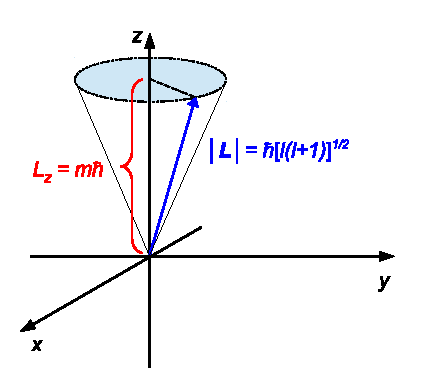
\includegraphics[scale=1]{vektorovymodel.eps}
\caption[Vektorový model momentu hybnosti]{Vektorový model momentu hybnosti. Protože jednotlivé složky vektoru momentu hybnosti spolu nekomutují, nemůžeme současně změřit více než jednu složku, konvenčně se volí $z$-ová složka. Ostatní složky, $x$-ová a $y$-ová, jsou tudíž neurčené, což se znázorňuje pomocí rotačního kužele. Velikost $|\mathbf{L}|$ vektoru momentu hybnosti komutuje se všemi složkami, proto je současně měřitelná spolu s~jednou složkou. To znamená, že o~vektoru momentu hybnosti z~měření dostaneme údaje o~velikosti a průmětu do $z$-ové osy. Prostorové kvantování momentu hybnosti je pak dáno vlastními čísly operátorů $\hat{L^2}$ a $\hat{L_z}$.}
\label{obr:VektorovyModel}
\end{figure}

Na průmětu 3D vektorového modelu, například do roviny $zy$, si můžeme graficky vysvětlit význam posuvných operátorů (obrázek~\ref{obr:ZebrickoveOperatory}). Operátor $\hat{L_+}$ posouvá kvantový stav $Y_l^m$ do nového stavu s~hodnotou kvantového čísla $m$ o~jedničku větší, tj. stavu $Y_l^{m+1}$. Na druhou stranu operátor  $\hat{L_-}$ posouvá kvantový stav $Y_l^m$ do nového stavu s~hodnotou kvantového čísla $m$ o~jedničku menší, tj. do stavu $Y_l^{(m-1)}$.
\begin{figure} [!ht]
\centering
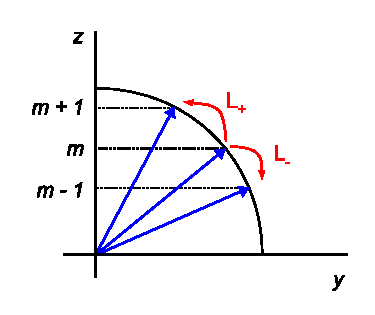
\includegraphics[scale=1]{zebrickoveoperatory.eps}
\caption[Posuvné operátory ve vektorovém modelu]{Činnost posuvných operátorů si můžeme představit tak, že operátor $\hat{L}_{+}$ mění kvantový stav $Y_l^m$ na kvantový stav $Y_l^{m+1}$ a operátor $\hat{L}_{-}$ mění kvantový stav $Y_l^m$ na stav $Y_l^{m-1}$.}
\label{obr:ZebrickoveOperatory}
\end{figure}

\subsection{Operátor momentu hybnosti v~polárních souřadnicích}
\label{kap:PolarniSouradnice}

Při popisu daného systému volíme takový souřadný systém, aby byl popis co možná nejjednodušší. V~případě přímočarého pohybu je nejvýhodnější souřadný systém pravoúhlých kartézských souřadnic $(x,y,z)$. Tento systém už ale není vhodný pro popis rotačních pohybů, protože popis křivosti je v~něm komplikovaný. Proto byly zavedeny křivočaré systémy souřadnic, které jednoduše popisují rotační pohyby.

Základní soustavou křivočarých souřadnic v~3D prostoru je sférická soustava $(r,\theta,\phi)$, kde $r$ je vzdálenost bodu od zvoleného počátku, $\theta$ je úhel, který svírá průvodič uvažovaného bod s~osou $z$ a $\phi$ je úhel, který svírá průvodič s~osou $x$. Abychom mohli přejít od kartézského souřadného systému do sférické souřadné soustavy, musíme odvodit transformační rovnice, které jednoznačně určují transformaci souřadnic $(x,y,z) \rightarrow (r,\theta,\phi)$. Z~geometrických úvah odvodíme transformační rovnice
\begin{equation}
x= r \sin \theta \cos \phi \mbox{,}
\label{rov:Hybnost39}
\end{equation}
\begin{equation}
y= r \sin \theta \sin \phi
\label{rov:Hybnost40}
\end{equation}
a
\begin{equation}
z = r \cos \theta \mbox{.}
\label{rov:Hybnost41}
\end{equation}
Obdobně odvodíme transformační rovnice pro inverzní transformaci $(r,\theta,\phi) \rightarrow (x,y,z)$
\begin{equation}
r^2=x^2+y^2+z^2 \mbox{,}
\label{rov:Hybnost42}
\end{equation}
\begin{equation}
\cos \theta = z/r
\label{rov:Hybnost43}
\end{equation}
a
\begin{equation}
\tan \phi = y/x \mbox{.}
\label{rov:Hybnost44}
\end{equation}

Dále nás bude zajímat, jaký způsobem se změní operátory momentu hybnosti, když od kartézských souřadnic přejdeme k~souřadnicím sférickým. Protože ve výrazech (\ref{rov:Hybnost6}), (\ref{rov:Hybnost7}) a (\ref{rov:Hybnost8}) pro operátory složek momentu hybnosti vystupují parciální derivace, nejprve si tyto derivace vyjádříme
\begin{equation}
\frac{\partial r}{\partial x} = \sin \theta \cos \phi, \quad \frac{\partial r}{\partial y} = \sin \theta \sin \phi, \quad \frac{\partial r}{\partial z} = \cos \theta \mbox{,}
\label{rov:Hybnost45}
\end{equation}
\begin{equation}
\frac{\partial \theta}{\partial x} = \frac{\cos \theta \cos \phi}{r}, \quad \frac{\partial \theta}{\partial y} = \frac{\cos \theta \sin \phi}{r}, \quad \frac{\partial \theta}{\partial z} = -\frac{\sin \theta}{r}
\label{rov:Hybnost46}
\end{equation}
a
\begin{equation}
\frac{\partial \phi}{\partial x} = -\frac{\sin \phi}{r \sin \theta}, \quad \frac{\partial \phi}{\partial y} = \frac{\cos \phi}{r \sin \theta}, \quad \frac{\partial \phi}{\partial z} = 0 \mbox{.}
\label{rov:Hybnost47}
\end{equation}
Pomocí vztahů (\ref{rov:Hybnost45}), (\ref{rov:Hybnost46}) a (\ref{rov:Hybnost47}) a pravidlu o~derivaci složené funkce odvodíme výrazy pro operátory složek momentu hybnosti ve sférických souřadnicích
\begin{equation}
\hat{L_x}= i \hbar \left( \sin \phi \frac{\partial}{\partial \theta} + \cot \theta \cos \phi \frac{\partial}{\partial \phi} \right) \mbox{,}
\label{rov:Hybnost48}
\end{equation}
\begin{equation}
\hat{L_y}= i \hbar \left( -\cos \phi \frac{\partial}{\partial \theta} + \cot \theta \sin \phi \frac{\partial}{\partial \phi} \right)
\label{rov:Hybnost49}
\end{equation}
a
\begin{equation}
\hat{L_z}= -i \hbar \frac{\partial}{\partial \phi} \mbox{.}
\label{rov:Hybnost50}
\end{equation}
Z~rovnice (\ref{rov:Hybnost50}) vidíme, proč se konvenčně pracuje se $z$-ovou složkou momentu hybnosti, protože její vyjádření ve sférických souřadnicích je nejjednodušší.

Když máme vyjádřeny jednotlivé operátory složek momentu hybnosti ve sférických souřadnicích, není problém vyjádřit ve sférických souřadnicích i operátor kvadrátu momentu hybnosti
\begin{equation}
\hat{L^2} = - \hbar^2 \left[ \frac{1}{\sin \theta} \frac{\partial}{\partial \theta} \left(\sin \theta \frac{\partial}{\partial \theta} \right) + \frac{1}{\sin^2 \theta}\frac{\partial^2}{\partial \phi^2} \right] \mbox{.}
\label{rov:Hybnost51}
\end{equation}

\subsection{Pohyb částice po kouli}
\label{kap:PohybCasticePoKouli}

V~tento okamžik máme potřebný aparát k~tomu, abychom mohli vyřešit problém pohybu částice s~momentem hybnosti. Naším cílem bude nalézt vlastní funkce $\psi(r, \theta, \phi)$ operátorů $\hat{L^2}$ a~$\hat{L_z}$. Tento jednoduchý problém nám poslouží  v~kapitole \ref{kap:vodik}, kde budeme řešit vodíkový atom.

Zapišme si nejprve vlastní problémy operátorů $\hat{L^2}$ a~$\hat{L_z}$
\begin{equation}
\hat{L^2}\psi(r, \theta, \phi) = l(l+1) \hbar^2 \psi(r, \theta, \phi)
\label{rov:Hybnost52}
\end{equation}
a
\begin{equation}
\hat{L_z}\psi(r, \theta, \phi) = m \hbar \psi(r, \theta, \phi) \mbox{,}
\label{rov:Hybnost53}
\end{equation}
kde jsme za vlastní čísla dosadili ze vztahů \eqref{rov:VlastniCislaKvadratu} a \eqref{rov:VlastniCislaZSlozky}. Protože operátor $\hat{L}^2$ ani operátor $\hat{L}_z$ nepůsobí na souřadnici $r$, můžeme provést separaci proměnných
\begin{equation}
\psi(r, \theta, \phi) = R(r) Y (\theta, \phi),
\label{rov:Hybnost54}
\end{equation}
kde $R(r)$ je radiální část vlnové funkce a $Y(\theta,\phi)$ je angulární část vlnové funkce, kterou označujeme jako sférické harmoniky. Díky separaci proměnných se problém pohybu částice v~3D prostoru rozpadl na pohyb částice po kulové sféře, popsaný pomocí sférické harmoniky a na vyšetření pohybu částice po daném orbitu ve vzdálenosti $r$ od zvoleného počátku, který je popsaný radiální částí vlnové funkce. Separace proměnných (\ref{rov:Hybnost54}) umožňuje zvlášť vyšetřit pohyb po kulové sféře a zvlášť radiální pohyb. V~tuto chvíli nás zajímá pouze pohyb po kulové sféře, proto budeme dále pracovat jen s~vlnovou funkcí ve tvaru sférické harmoniky $Y(\theta, \phi)$.

Operátor $\hat{L_z}$ působí pouze na souřadnici $\phi$ (viz vztah (\ref{rov:Hybnost50})), proto můžeme předpokládat, že i sférické harmoniky můžeme separovat
\begin{equation}
Y(\theta, \phi) = \Theta (\theta) \Phi (\phi) \mbox{.}
\label{rov:Hybnost55}
\end{equation}

Vyřešme nejprve vlastní problém (\ref{rov:Hybnost53}), kde za operátor $\hat{L_z}$ dosadíme ze vztahu (\ref{rov:Hybnost50}) a~dále využijeme separaci proměnných (\ref{rov:Hybnost55})
\begin{equation}
-i \hbar \Theta \frac{\partial \Phi}{\partial \phi} = m \hbar \Theta \Phi \mbox{.}
\label{rov:Hybnost56}
\end{equation}
Rovnici dále upravme
\begin{equation}
-i  \frac{\mathrm{d} \Phi}{\Phi} = m \mathrm{d} \phi
\label{rov:Hybnost57}
\end{equation}
a dostaneme obyčejnou diferenciální rovnici pro $\Phi(\phi)$. Integrací rovnice (\ref{rov:Hybnost57}) získáme řešení ve tvaru
\begin{equation}
\Phi = A e^{i m \phi} \mbox{,}
\label{rov:Hybnost58}
\end{equation}
kde $A$ je integrační konstanta. Tu určíme z~normovací podmínky
\begin{equation}
\int_{0}^{2\pi} \Phi^{\ast}\Phi \mathrm{d} \phi \stackrel{a}{=} A^2 \int_{0}^{2\pi} \mathrm{d} \phi = 2 A^2 \pi = 1 \Rightarrow A = \frac{1}{\sqrt{2 \pi}} \mbox{.}
\label{rov:Hybnost59}
\end{equation}
Úprava $a$ plyne z~následujícího
\begin{equation}
\Phi^{\ast}\Phi = e^{-i m \phi}e^{i m \phi}=e^0=1 \mbox{.}
\label{rov:Hybnost60}
\end{equation}
Integrační meze ve vztahu (\ref{rov:Hybnost59}) plynou z~toho, že ve sférických souřadnicích platí $\phi \in \langle 0;2\pi\rangle$. Sférickou harmoniku $Y(\theta, \phi)$ tak můžeme zapsat jako
\begin{equation}
Y(\theta, \phi) = \Theta(\theta) \Phi(\phi) = \Theta(\theta) \frac{1}{2\pi}e^{im\phi} \mbox{.}
\label{rov:Hybnost61}
\end{equation}

Dosazením sférické harmoniky (\ref{rov:Hybnost61}) do vlastního problému (\ref{rov:Hybnost52}) operátoru $\hat{L^2}$ a řešením vzniknuvší diferenciální rovnice bychom došli k~závěru, že se jedná o~typ diferenciální rovnice, která se řeší pomocí ortogonálních polynomů, konkrétně pomocí přidružených Lagendrových polynomů $S_l^{|m|}(\cos \theta)$. Pak se ukáže, že platí
\begin{equation}
\Theta(\cos \theta) \equiv S_l^{|m|} (\cos \theta) \mbox{.}
\label{rov:Hybnost62}
\end{equation}
Výslednou sférickou harmoniku $Y_l^{m}$ tak můžeme zapsat ve tvaru
\begin{equation}
\boxed{Y_l^{m}(\theta, \phi) = N_{lm} S_l^{|m|} (\cos \theta) e^{i m \phi} \mbox{,}}
\label{rov:Hybnost63}
\end{equation}
kde $N_{lm}$ je normovací faktor
\begin{equation}
N_{lm} = \sqrt{\frac{(l-|m|)! (2l+1)}{4\pi(l+|m|)!}}\mbox{.}
\label{rov:Hybnost64}
\end{equation}

Závěr našeho snažení je následující. Pohyb částice po kulové sféře můžeme popsat pomocí sférických harmonik, neboli angulární část vlnové funkce $\psi(r,\theta,\phi)$. Sférické harmoniky $Y_l^{m}(\theta, \phi)$ závisí pouze na úhlech $\theta$ a $\phi$ a jsou parametrizovány dvojicí kvantových číslech $l$ a $m$. Obecně se jedná o~komplexní funkce, na jejichž zobrazení bychom potřebovali 6-ti dimenzionální prostor (jedná se o~3D funkce v~komplexní rovině). Proto nezobrazujeme přímo sférické harmoniky, ale jejich lineární kombinace.

\subsection{Energie pohybu po sféře}
\label{kap:EnergiePohybSfera}

Budeme-li chtít určit energii částice, která se pohybuje po kulové sféře, zapíšeme vlastní problém pro energii, tj. Schrödingerovu rovnici s~hamiltoniánem ve tvaru
\begin{equation}
\hat{H} = -\frac{\hbar^2}{2m}\nabla^2 \mbox{,}
\label{rov:Hybnost65}
\end{equation}
kde předpokládáme, že částice se nepohybuje v~žádném potenciálu, tj. $V=0$. Protože hamiltonián $\hat{H}$ komutuje s~operátory $\hat{L^2}$ a $\hat{L_z}$, mají tyto operátory společný soubor vlastních funkcí, kterými jsou sférické harmoniky $Y_l^m$.

Budeme postupovat tak, že si operátor $\nabla^2$ vyjádříme ve sférických souřadnicích
\begin{equation}
\nabla^2 = \frac{\partial^2}{\partial r^2} + \frac{2}{r}\frac{\partial}{\partial r} + \frac{1}{r^2}\Lambda^2 \mbox{,}
\label{rov:Hybnost66}
\end{equation}
kde operátor $\Lambda^2$ je legendrián, který představuje angulární část operátoru $\nabla^2$
\begin{equation}
\Lambda^2 = \frac{1}{\sin^2 \theta}\frac{\partial^2}{\partial \phi^2} + \frac{1}{\sin \theta}\frac{\partial}{\partial \theta}\sin \theta \frac{\partial}{\partial \theta}\mbox{.}
\label{rov:Hybnost67}
\end{equation}
Protože nás zajímá pouze pohyb po kulové sféře, kde se nemění souřadnice $r$ zredukuje se operátor $\nabla^2$ na $\Lambda^2$. Uvědomíme-li si, že moment setrvačnosti je definován jako $I=mr^2$, můžeme Schrödingerovu rovnici pro pohyb na kulové ploše zapsat jako
\begin{equation}
\Lambda^2 Y_l^m = - \frac{2 I E}{\hbar^2} Y_l^m \mbox{.}
\label{rov:Hybnost68}
\end{equation}
Dále je možné ukázat, že platí 
\begin{equation}
\Lambda^2 Y_l^m = -l(l+1) Y_l^m \mbox{.}
\label{rov:Hybnost69}
\end{equation}
Porovnáním rovnic (\ref{rov:Hybnost68}) a (\ref{rov:Hybnost69}) dostaneme pro energii
\begin{equation}
\boxed{E_{lm} = l(l+1)\frac{\hbar^2}{2I} \mbox{,}}
\label{rov:Hybnost70}
\end{equation}
kde každý energetický stav $E_{lm}$ je $2l+1$ degenerovaný.

\begin{priklad}
\textbf{Zadání}: Délky vazeb jsou určovány ze spektroskopických měření, která jsou velice přesná. Z rotačního spektra HCl jsme odvodili, že $B=10{,}59342$~cm$^{-1}$. Hmotnosti $^1$H a $^{35}$Cl jsou $1{,}0078250$ a $34{,}9688527$~a.u. Odvoďte délku vazby v molekule HCl.\\[0.1cm]
\textbf{Řešení:} Pro rotační konstantu $B$ platí
\begin{displaymath}
B = \frac{h}{8 \pi^2 \mu c r_0^2},
\end{displaymath} 
kde $\mu$ je redukovaná hmotnost. Pak
\begin{displaymath}
r_0 = \sqrt{\frac{h}{8 \pi^2 \mu c B}} = 1{,}274553 \cdot 10^{-10} \mbox{ m}.
\end{displaymath} \vspace{-0.7cm}
\end{priklad}